\documentclass[11pt]{article}
\usepackage[textwidth=18.0cm, textheight=23.0cm, top=2.0cm]{geometry}
\usepackage{pst-all}
\usepackage{amssymb}
\usepackage{tikz}
\usepackage{underscore}\begin{document}
\pagestyle{empty}


ClassName: \underline{\textbf{Class_08.2bp-0}}
\par
BinSize: \underline{\textbf{100 × 100}}
\par
ReduceSize: \underline{\textbf{99 × 100}}
\par
TypeNum: \underline{\textbf{19}}
\par
Num: \underline{\textbf{20}}
\par
OutS: \underline{\textbf{60000}}
\par
InS: \underline{\textbf{48363}}
\par
Rate: \underline{\textbf{0.806}}
\par
UB: \underline{\textbf{6}}
\par
LB0: \underline{\textbf{6}}
\par
LB: \underline{\textbf{6}}
\par
LBWithCut: \underline{\textbf{6}}
\par
NodeCut: \underline{\textbf{0}}
\par
ExtendedNodeCnt: \underline{\textbf{1}}
\par
GenNodeCnt: \underline{\textbf{1}}
\par
PrimalNode: \underline{\textbf{0}}
\par
ColumnCount: \underline{\textbf{6}}
\par
TotalCutCount: \underline{\textbf{0}}
\par
RootCutCount: \underline{\textbf{0}}
\par
LPSolverCnt: \underline{\textbf{1}}
\par
PricingSolverCnt: \underline{\textbf{0}}
\par
BranchAndBoundNum: \underline{\textbf{1}}
\par
isOpt: \underline{\textbf{true}}
\par
TimeOnInitSolution: \underline{\textbf{600.000 s}}
\par
TimeOnPrimal: \underline{\textbf{0.000 s}}
\par
TimeOnPricing: \underline{\textbf{0.000 s}}
\par
TimeOnRmp: \underline{\textbf{0.063 s}}
\par
TotalTime: \underline{\textbf{600.297 s}}
\par
\newpage


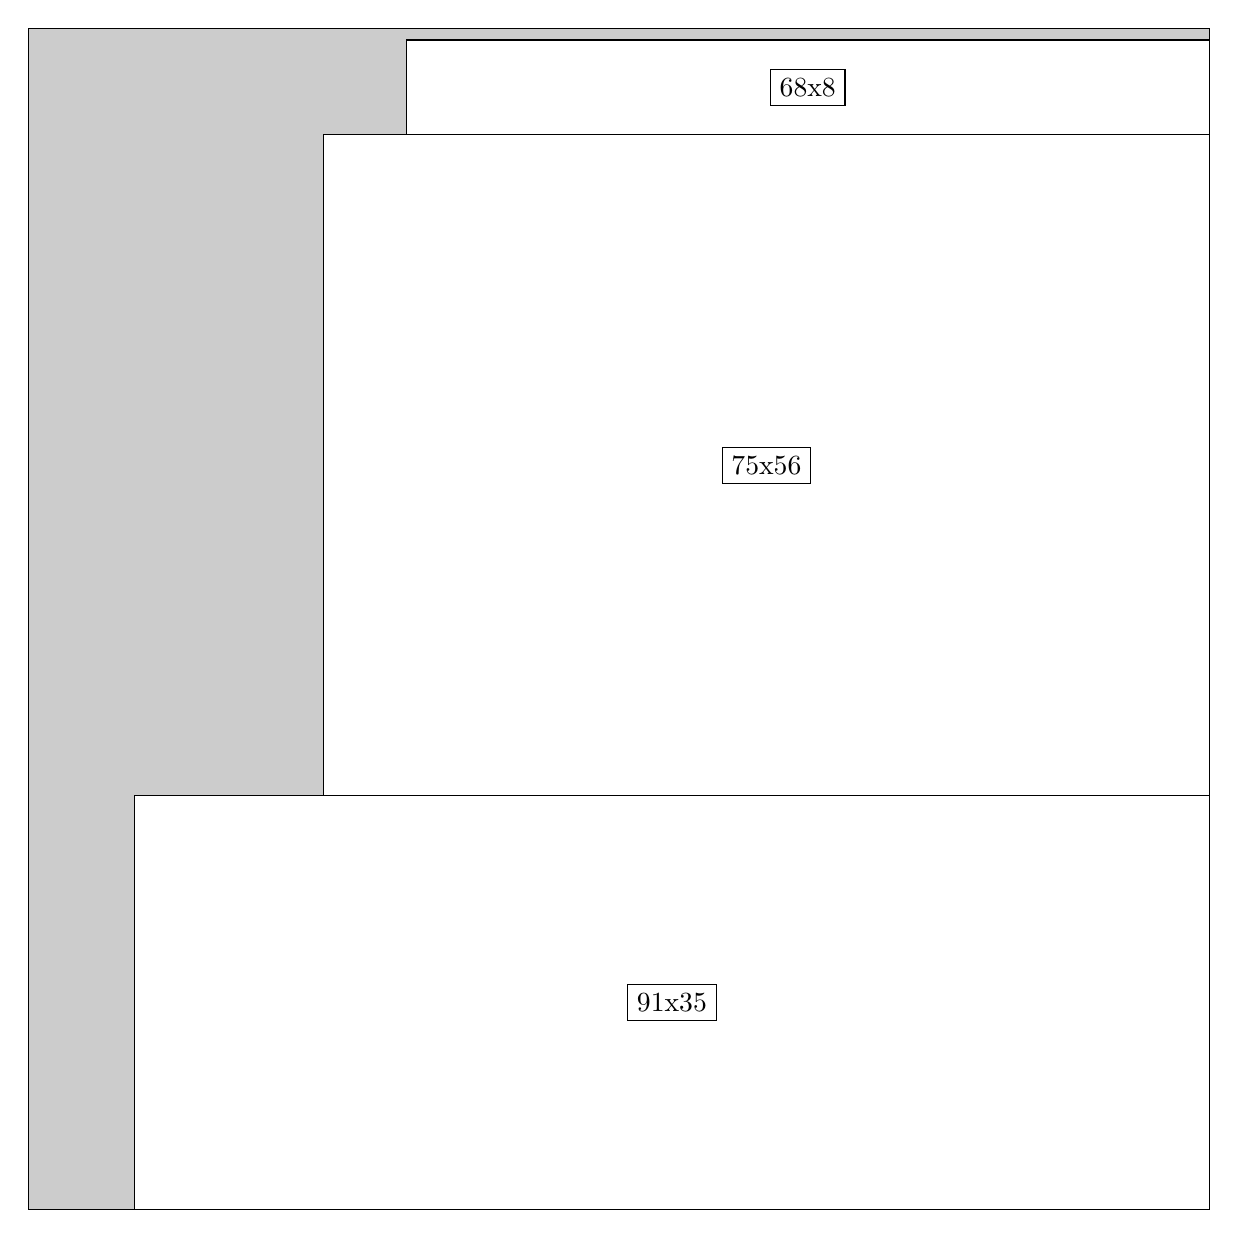
\begin{tikzpicture}[shorten >=1pt,scale=1.0,every node/.style={scale=1.0},->]
\tikzstyle{vertex}=[circle,fill=black!25,minimum size=14pt,inner sep=0pt]
\filldraw[fill=gray!40!white, draw=black] (0,0) rectangle (15.0,15.0);
\foreach \name/\x/\y/\w/\h in {91x35/1.3499999999999999/0.0/13.65/5.25,75x56/3.75/5.25/11.25/8.4,68x8/4.8/13.65/10.2/1.2}
\filldraw[fill=white!40!white, draw=black] (\x,\y) rectangle node[draw] (\name) {\name} ++(\w,\h);
\end{tikzpicture}


w =91 , h =35 , x =9 , y =0 , v =3185
\par
w =75 , h =56 , x =25 , y =35 , v =4200
\par
w =68 , h =8 , x =32 , y =91 , v =544
\par
\newpage


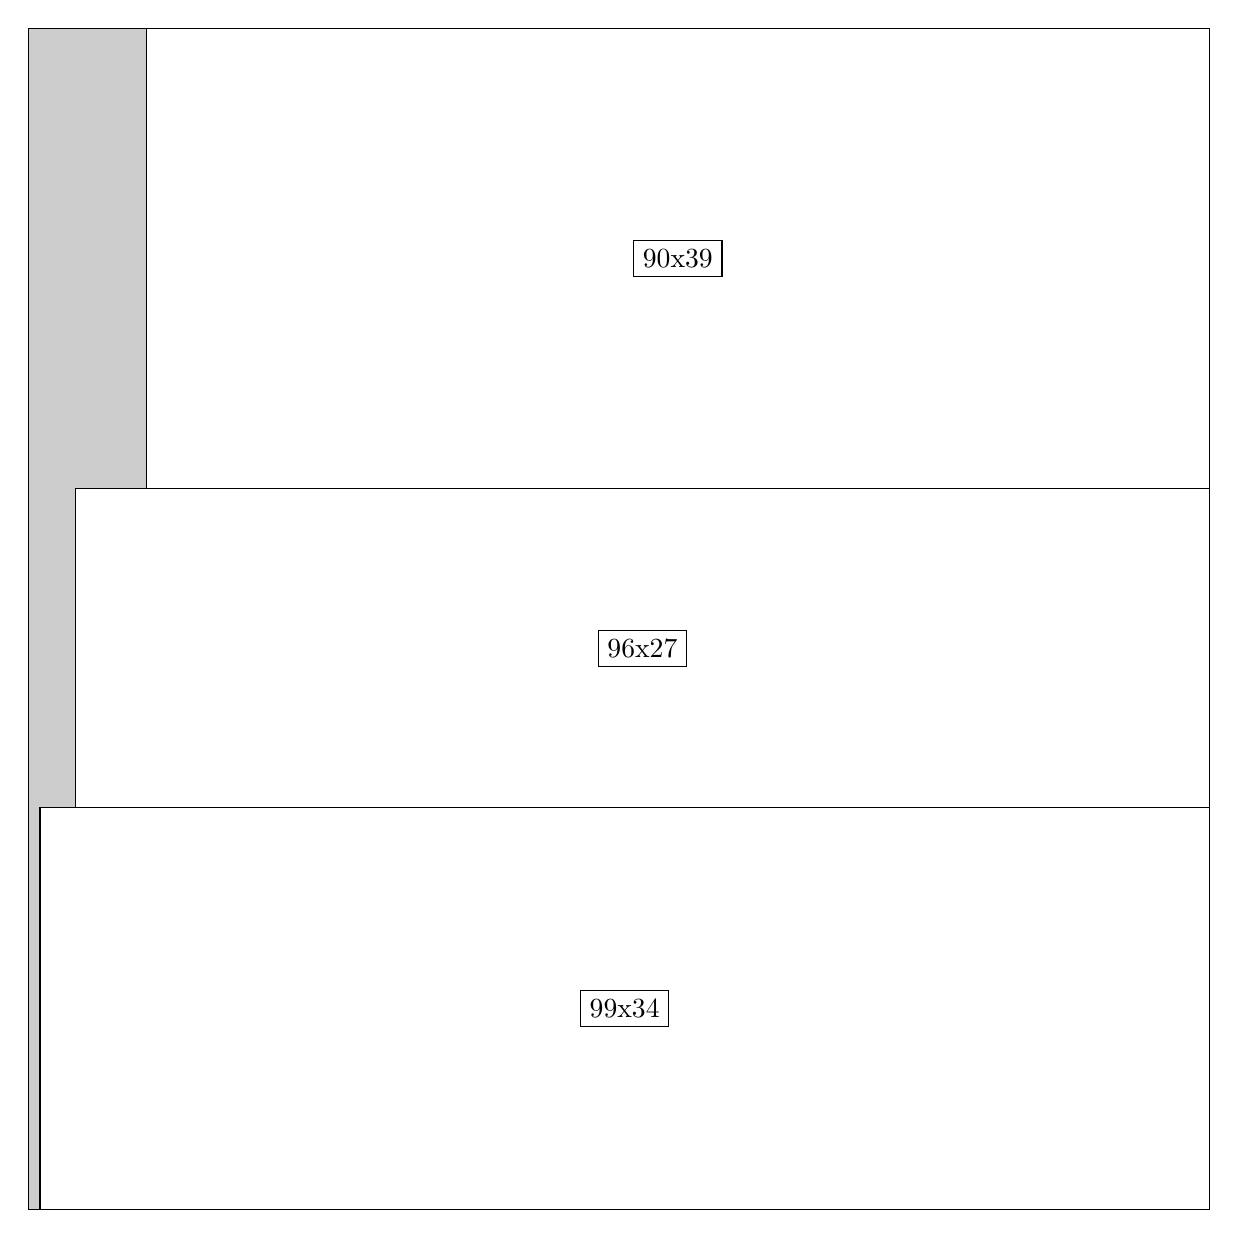
\begin{tikzpicture}[shorten >=1pt,scale=1.0,every node/.style={scale=1.0},->]
\tikzstyle{vertex}=[circle,fill=black!25,minimum size=14pt,inner sep=0pt]
\filldraw[fill=gray!40!white, draw=black] (0,0) rectangle (15.0,15.0);
\foreach \name/\x/\y/\w/\h in {99x34/0.15/0.0/14.85/5.1,96x27/0.6/5.1/14.399999999999999/4.05,90x39/1.5/9.15/13.5/5.85}
\filldraw[fill=white!40!white, draw=black] (\x,\y) rectangle node[draw] (\name) {\name} ++(\w,\h);
\end{tikzpicture}


w =99 , h =34 , x =1 , y =0 , v =3366
\par
w =96 , h =27 , x =4 , y =34 , v =2592
\par
w =90 , h =39 , x =10 , y =61 , v =3510
\par
\newpage


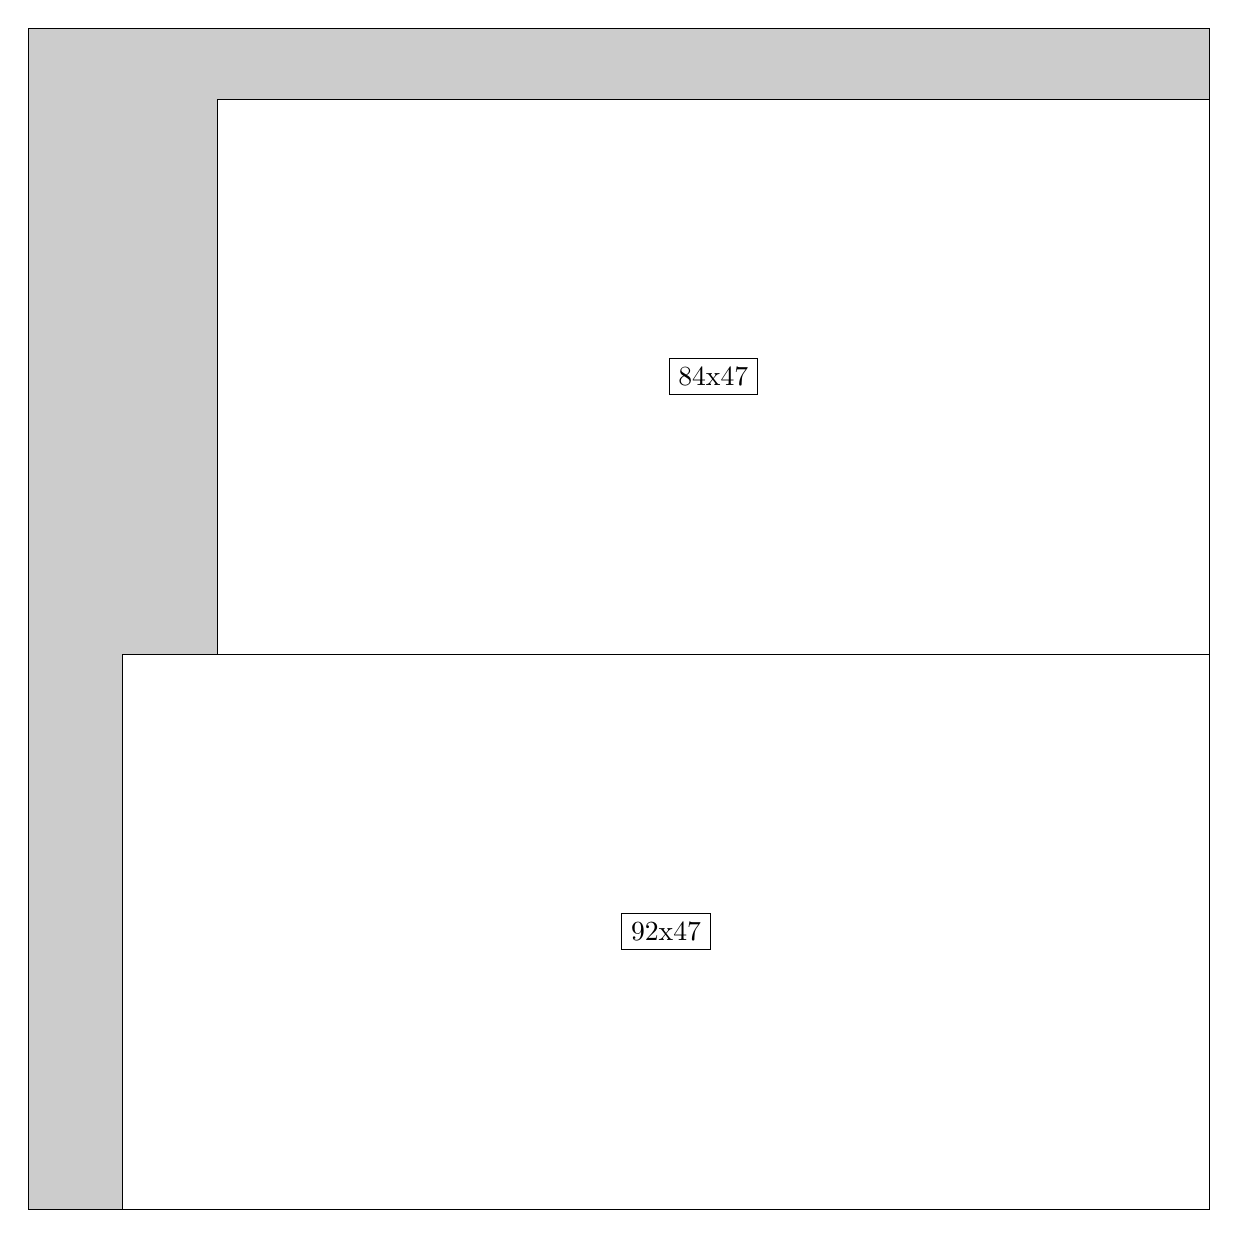
\begin{tikzpicture}[shorten >=1pt,scale=1.0,every node/.style={scale=1.0},->]
\tikzstyle{vertex}=[circle,fill=black!25,minimum size=14pt,inner sep=0pt]
\filldraw[fill=gray!40!white, draw=black] (0,0) rectangle (15.0,15.0);
\foreach \name/\x/\y/\w/\h in {92x47/1.2/0.0/13.799999999999999/7.05,84x47/2.4/7.05/12.6/7.05}
\filldraw[fill=white!40!white, draw=black] (\x,\y) rectangle node[draw] (\name) {\name} ++(\w,\h);
\end{tikzpicture}


w =92 , h =47 , x =8 , y =0 , v =4324
\par
w =84 , h =47 , x =16 , y =47 , v =3948
\par
\newpage


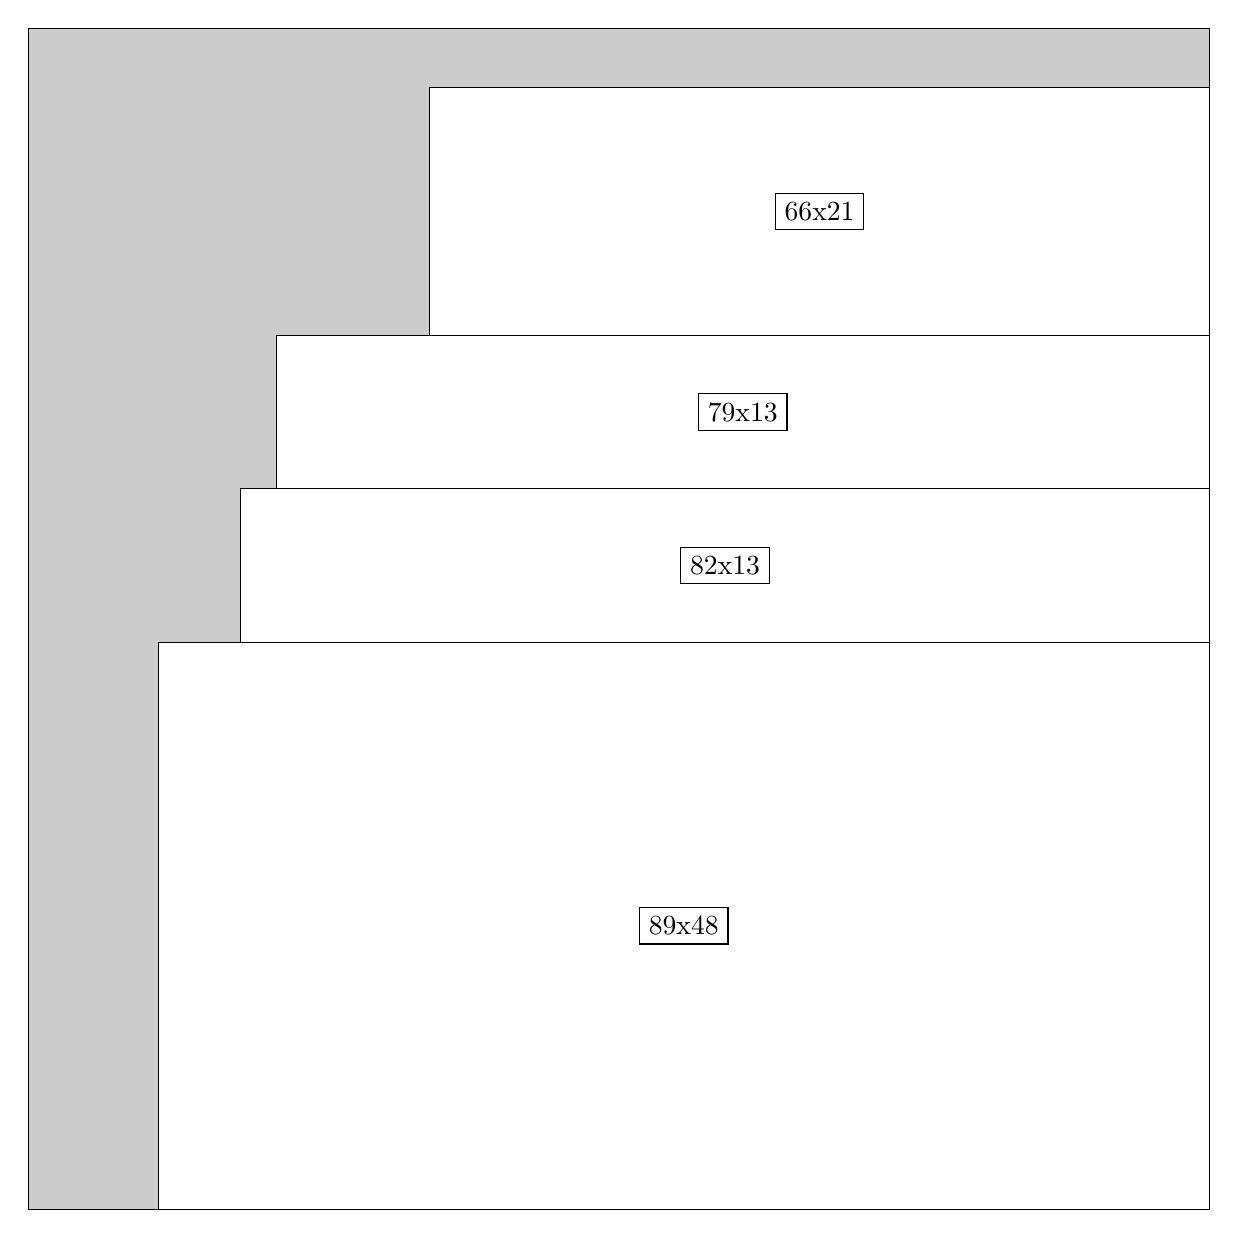
\begin{tikzpicture}[shorten >=1pt,scale=1.0,every node/.style={scale=1.0},->]
\tikzstyle{vertex}=[circle,fill=black!25,minimum size=14pt,inner sep=0pt]
\filldraw[fill=gray!40!white, draw=black] (0,0) rectangle (15.0,15.0);
\foreach \name/\x/\y/\w/\h in {89x48/1.65/0.0/13.35/7.199999999999999,82x13/2.6999999999999997/7.199999999999999/12.299999999999999/1.95,79x13/3.15/9.15/11.85/1.95,66x21/5.1/11.1/9.9/3.15}
\filldraw[fill=white!40!white, draw=black] (\x,\y) rectangle node[draw] (\name) {\name} ++(\w,\h);
\end{tikzpicture}


w =89 , h =48 , x =11 , y =0 , v =4272
\par
w =82 , h =13 , x =18 , y =48 , v =1066
\par
w =79 , h =13 , x =21 , y =61 , v =1027
\par
w =66 , h =21 , x =34 , y =74 , v =1386
\par
\newpage


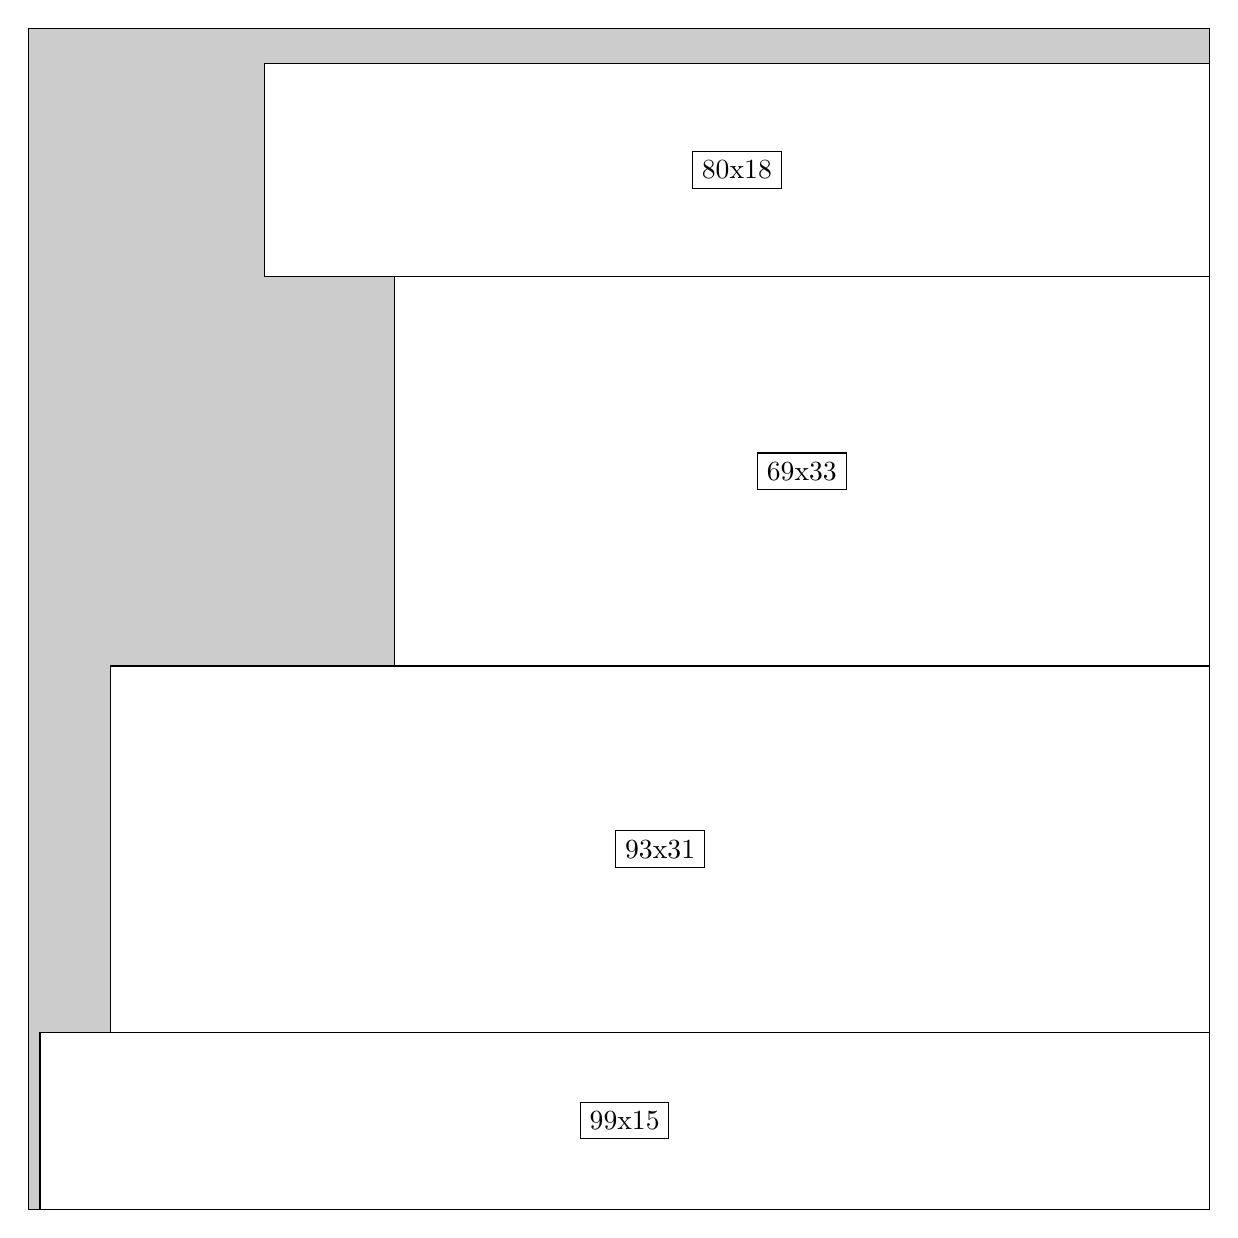
\begin{tikzpicture}[shorten >=1pt,scale=1.0,every node/.style={scale=1.0},->]
\tikzstyle{vertex}=[circle,fill=black!25,minimum size=14pt,inner sep=0pt]
\filldraw[fill=gray!40!white, draw=black] (0,0) rectangle (15.0,15.0);
\foreach \name/\x/\y/\w/\h in {99x15/0.15/0.0/14.85/2.25,93x31/1.05/2.25/13.95/4.6499999999999995,69x33/4.6499999999999995/6.8999999999999995/10.35/4.95,80x18/3.0/11.85/12.0/2.6999999999999997}
\filldraw[fill=white!40!white, draw=black] (\x,\y) rectangle node[draw] (\name) {\name} ++(\w,\h);
\end{tikzpicture}


w =99 , h =15 , x =1 , y =0 , v =1485
\par
w =93 , h =31 , x =7 , y =15 , v =2883
\par
w =69 , h =33 , x =31 , y =46 , v =2277
\par
w =80 , h =18 , x =20 , y =79 , v =1440
\par
\newpage


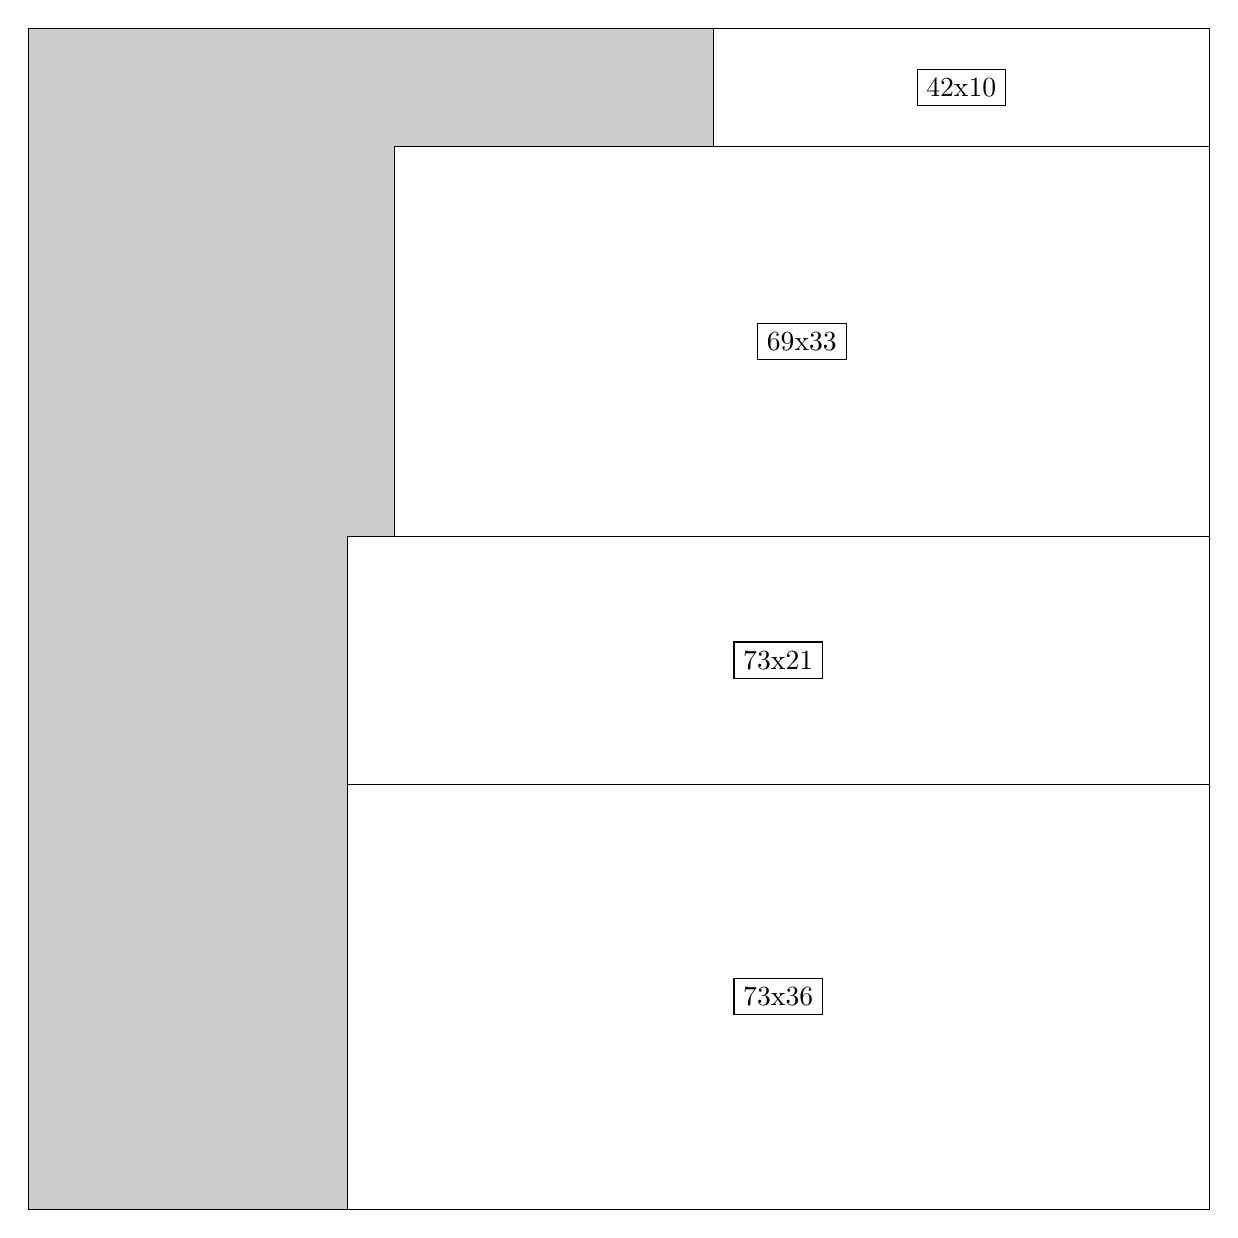
\begin{tikzpicture}[shorten >=1pt,scale=1.0,every node/.style={scale=1.0},->]
\tikzstyle{vertex}=[circle,fill=black!25,minimum size=14pt,inner sep=0pt]
\filldraw[fill=gray!40!white, draw=black] (0,0) rectangle (15.0,15.0);
\foreach \name/\x/\y/\w/\h in {73x36/4.05/0.0/10.95/5.3999999999999995,73x21/4.05/5.3999999999999995/10.95/3.15,69x33/4.6499999999999995/8.549999999999999/10.35/4.95,42x10/8.7/13.5/6.3/1.5}
\filldraw[fill=white!40!white, draw=black] (\x,\y) rectangle node[draw] (\name) {\name} ++(\w,\h);
\end{tikzpicture}


w =73 , h =36 , x =27 , y =0 , v =2628
\par
w =73 , h =21 , x =27 , y =36 , v =1533
\par
w =69 , h =33 , x =31 , y =57 , v =2277
\par
w =42 , h =10 , x =58 , y =90 , v =420
\par
\newpage


\end{document}